\begin{minipage}[c]{\textwidth}
\advance\leftskip-2.5cm
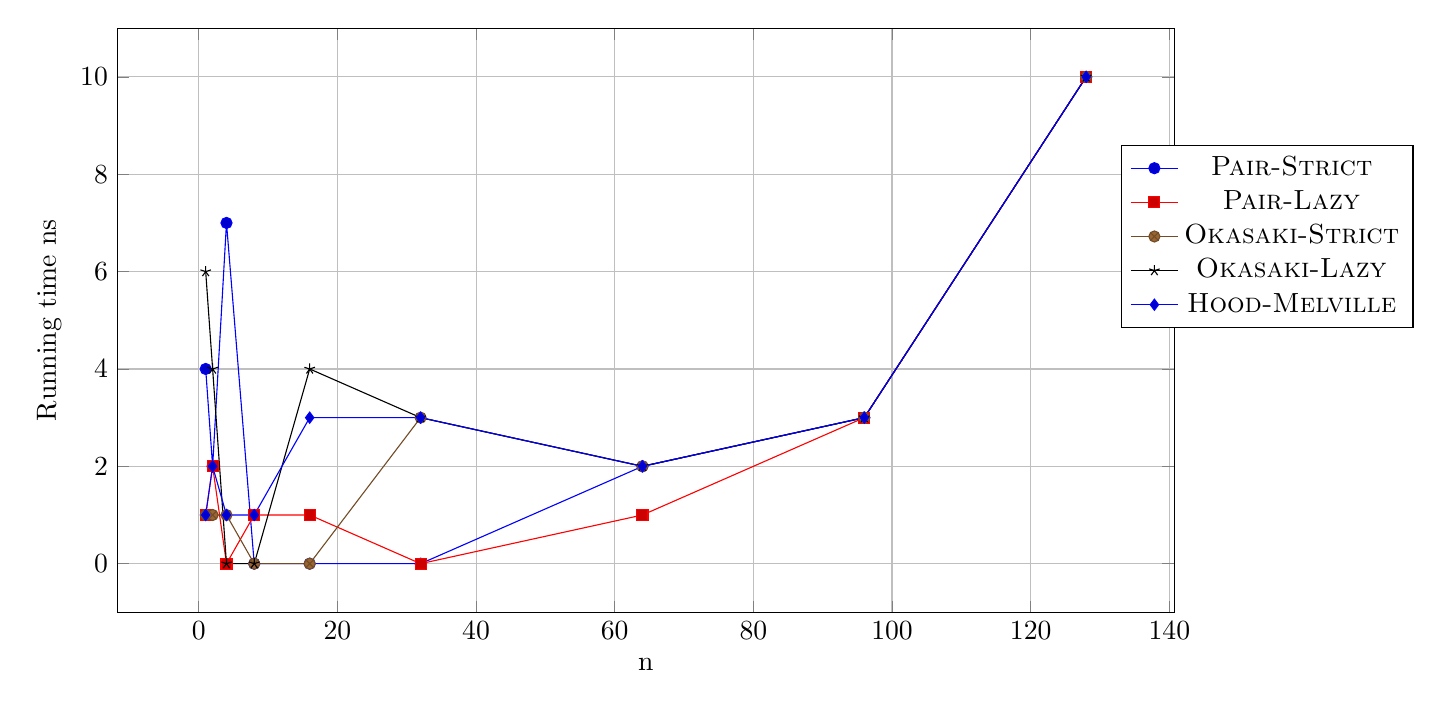
\begin{tikzpicture}
        \begin{axis}[
            xlabel = n,
            ylabel = Running time ns,
            height=9cm,
            width=15cm,
            grid=major,
            legend style={
            at={(0.95,0.8)},
            anchor=north west}]            
            legend pos=center west
    	]
    		
  
                \addplot coordinates {
(1,4)
(2,2)
(4,7)
(8,0)
(16,0)
(32,0)
(64,2)
(96,3)
(128,10)

    	};
        
    	\addlegendentry{\textsc{Pair-Strict}}

        \addplot coordinates {
(1,1)
(2,2)
(4,0)
(8,1)
(16,1)
(32,0)
(64,1)
(96,3)
(128,10)

    	};
        
    	\addlegendentry{\textsc{Pair-Lazy}}

        \addplot coordinates {
(1,1)
(2,1)
(4,1)
(8,0)
(16,0)
(32,3)
(64,2)
(96,3)
(128,10)

    	};
        
    	\addlegendentry{\textsc{Okasaki-Strict}}

        \addplot coordinates {
(1,6)
(2,4)
(4,0)
(8,0)
(16,4)
(32,3)
(64,2)
(96,3)
(128,10)

    	};
        
    	\addlegendentry{\textsc{Okasaki-Lazy}}

        \addplot coordinates {
(1,1)
(2,2)
(4,1)
(8,1)
(16,3)
(32,3)
(64,2)
(96,3)
(128,10)

    	};

    	\addlegendentry{\textsc{Hood-Melville}}

        \end{axis}

    \end{tikzpicture}
    \captionof{figure}{Time of merging $n$ queues with $n$ elements into a single queue divided by $n^3$}
    \label{fig:sample_figure}
\end{minipage}
